\begin{frame}{Robust nonrandom connectivity patterns}
  % 
  \begin{columns}
    % 
    \begin{column}{.45\textwidth}
      \minipage[c][0.75\textheight][s]{\columnwidth}
      
      \begin{figure}
        \centering
        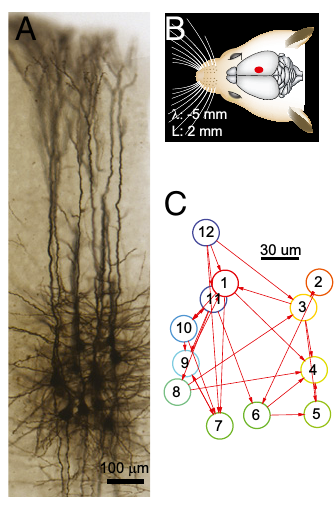
\includegraphics[width=\textwidth]{%
          figures/Perin2011_Fig1ABC.png} %
      \end{figure}
      

      
      \endminipage      
    \end{column}
    % 
    \begin{column}{.55\textwidth}


      \vspace{-0.2cm}
      
      \begin{figure}
        \centering
        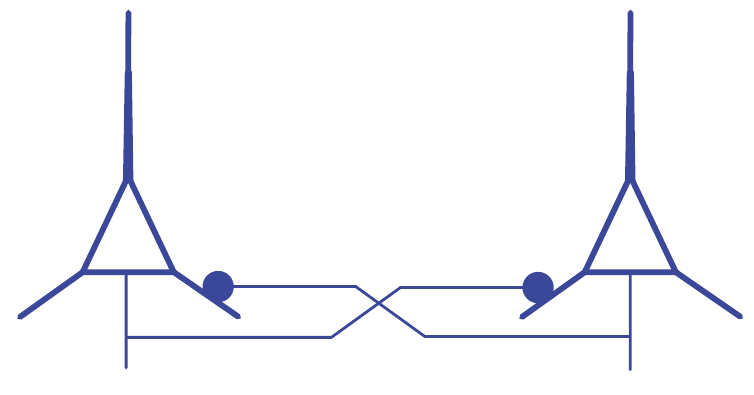
\includegraphics[width=0.525\textwidth]{%
          figures/two_neuron.png} %
      \end{figure}

      \vfill
      

      \begin{figure}
        \centering
        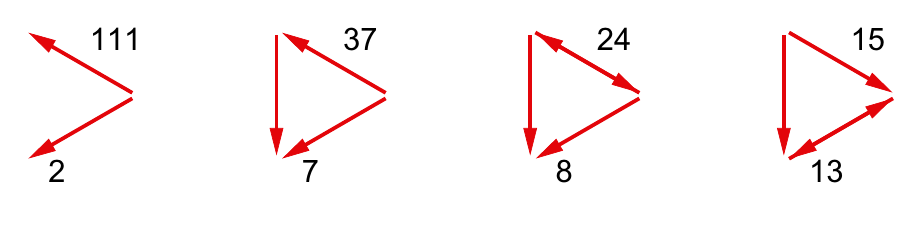
\includegraphics[width=\textwidth]{%
        figures/Perin2011_FigS2_custom.png} %
      \end{figure}

      \vfill
      

      \begin{figure}
        \centering
        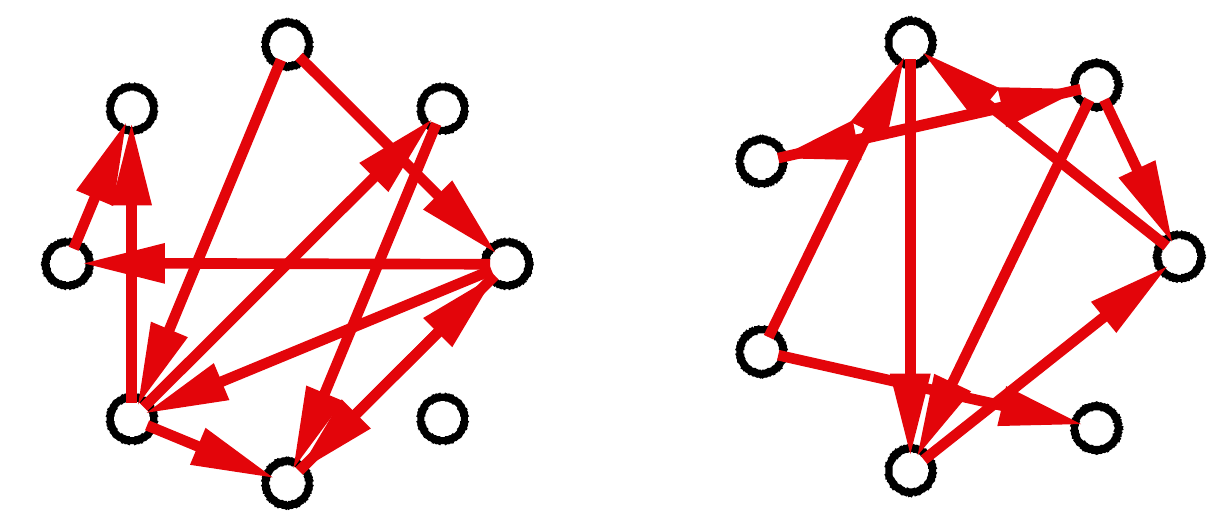
\includegraphics[width=0.7\textwidth]{%
          figures/clust_all.png} %
      \end{figure}
      
      \vfill

      
    \end{column}
  \end{columns}

  \source{\cite{Perin2011, Song2005, Markram1997, Miner2016, Gal2017,
      Vegue2017}}

  \pnote{
    
  }
  
\end{frame}



\begin{frame}{Connection counts in neuron clusters}

  \only<1>{
  \begin{figure}
    \centering
    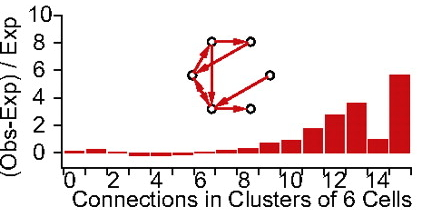
\includegraphics[width=0.85\textwidth]{%
      figures/perin_select6.png} %
  \end{figure}}
  

\only<2>{
  \begin{figure}
    \centering
    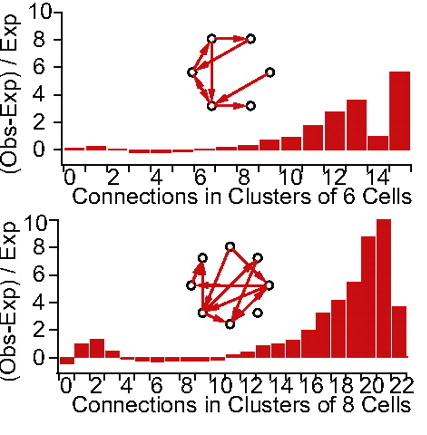
\includegraphics[width=0.625\textwidth]{%
      figures/perin_select2.png} %
  \end{figure}  }

\onslide<1-2>{\source{\cite{Perin2011}}}

% \only<3>{
%   \begin{figure}
%     \centering
%     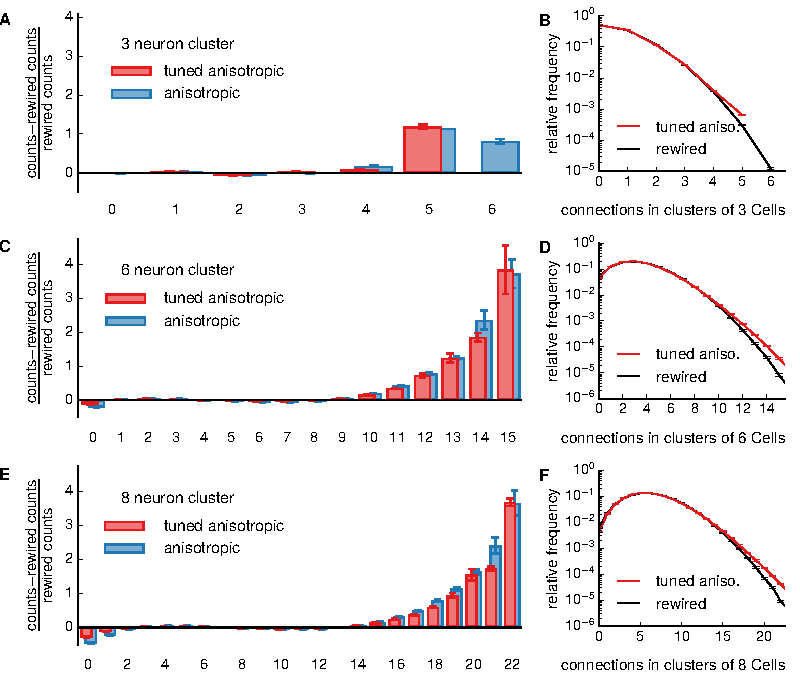
\includegraphics[width=0.925\textwidth]{%
%       figures/nc6_3c-3f_6c-6f_8c-8f.pdf} %
%   \end{figure}  }

  
\end{frame}


\begin{frame}{Connection counts in neuron clusters}

    \only<1>{
  \begin{figure}
    \centering
    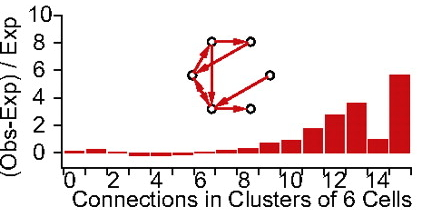
\includegraphics[width=0.625\textwidth]{%
      figures/perin_select6.png} %
  \end{figure}}


  \begin{figure}
    \centering
    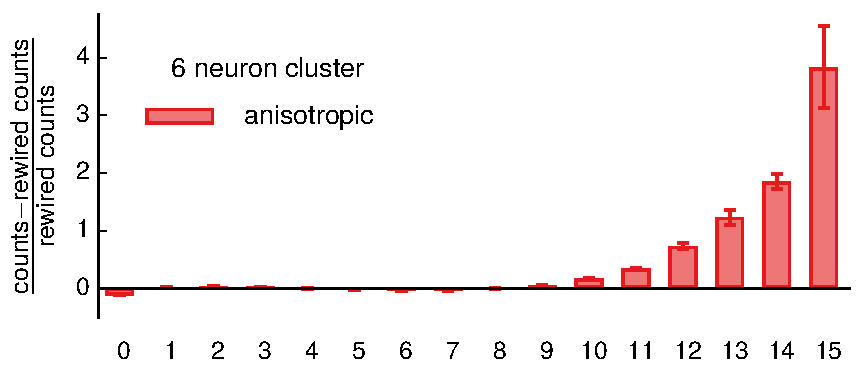
\includegraphics[width=0.875\textwidth]{%
    /home/fh/sci/lab/aniso_netw/ploscb_18/fig/slides/fig5C_6cluster_counts.pdf} %
  \end{figure} 
  
\end{frame}


\begin{frame}{Connection counts in neuron clusters}

  \vspace{0.1cm}
    \only<1>{
  \begin{figure}
    \centering
    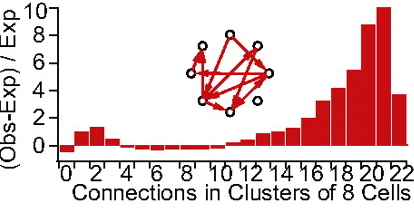
\includegraphics[width=0.625\textwidth]{%
      figures/8cluster_perin.png} %
  \end{figure}}

  \vspace{-0.5cm}

  \begin{figure}
    \centering
    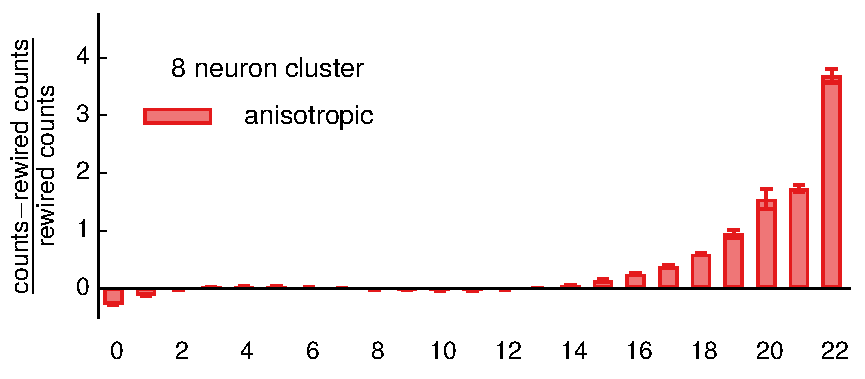
\includegraphics[width=0.875\textwidth]{%
    /home/fh/sci/lab/aniso_netw/ploscb_18/fig/slides/fig5E_8cluster_counts.pdf} %
  \end{figure} 
  
\end{frame}
